\section{Durso}\label{durso}

Tags: PC Alias: L'emule Creatore: Luca Giocatore: Luca Ispirazione:
Barbara D'Urso Luogo: Azura Razza: Mezzorco Classe: Barbaro Livello: 5

\section{Durso}\label{durso-1}

\begin{center}\rule{0.5\linewidth}{0.5pt}\end{center}

\begin{figure}
\centering

\includegraphics{Durso.png}
\caption{Durso.png}
\end{figure}

Informazioni Generali

Età:

Anno di nascita:

Paese di nascita:

Razza: Mezzorco

Relazioni:

Alleati:

Nemesi:

Possedimenti importanti:

\begin{center}\rule{0.5\linewidth}{0.5pt}\end{center}

\subsection{1. Descrizione Generale}\label{descrizione-generale}

\begin{center}\rule{0.5\linewidth}{0.5pt}\end{center}

\begin{figure}
\centering
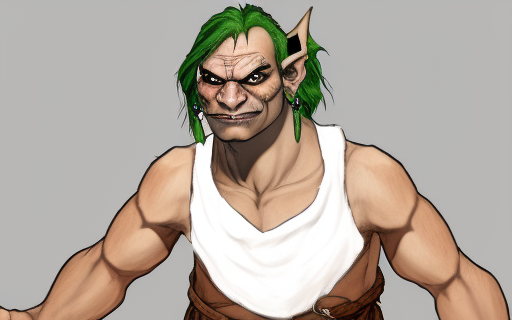
\includegraphics{a-fantasy-orc-that-looks-like-a-male-version-of-barbara-durso-.png}
\caption{a-fantasy-orc-that-looks-like-a-male-version-of-barbara-durso-.png}
\end{figure}

Durso è cresciuto in una tribù di orchi nel cuore della giungla. Fin da
piccolo, si è distinto per la sua stazza imponente e la sua forza
sovrumana. Nonostante l'aspetto minaccioso della sua razza, Durso ha
sempre avuto un cuore buono e un'innata propensione per aiutare gli
altri. Questo lo ha portato spesso a conflitti con gli altri membri
della tribù, che lo consideravano troppo morbido e indulgente.

Un giorno, durante una battuta di caccia, Durso e alcuni compagni della
tribù hanno incontrato un gruppo di avventurieri umani. Durso ha subito
trovato un'affinità con questi stranieri, che non lo giudicavano in base
alla sua razza. Ha iniziato a passare sempre più tempo con loro,
imparando il loro linguaggio e le loro usanze. L'usanza preferita di
Durso era quella nota come ``Postmeridiem V'', secondo la quale tutti si
sedevano attorno ad un fuoco a discutere in maniera semi-seria sui fatti
di cronaca del villaggio.

Con il tempo, Durso ha capito che il suo posto non era nella tribù degli
orchi, ma tra gli avventurieri. Ha lasciato la giungla e si è unito al
gruppo umano, diventando un ciarlatano e uno scaramantico. A volte fa
anche dei riti strani contro la sfortuna, credendo che possano aiutarlo
ad avere successo nelle sue imprese.

La collana di peperoncini che indossa al collo è un talismano che ha
ricevuto da un vecchio sciamano della sua tribù, che gli ha detto che
avrebbe portato fortuna. Durso la porta sempre con sé, convinto che sia
stata la chiave del suo successo come avventuriero.

Nostante la sua parlata un po' rozza, Durso ha un lato più profondo e
riflessivo. Ogni tanto, quando il gruppo si ferma per riposare dopo una
dura avventura, Durso comincia a filosofeggiare e a fare discorsi che
sorprendono i suoi compagni. Proprio come Barbara d'Urso, Durso ha la
capacità di trasformare temi apparentemente banali in riflessioni più
profonde sulla vita e sull'umanità. Anche se a volte i suoi discorsi
possono sembrare un po' strani, i suoi compagni lo rispettano per la sua
saggezza e la sua capacità di vedere le cose da diverse prospettive.

Durso è un buon compagno di squadra e un difensore appassionato dei più
deboli. Anche se non sempre segue le regole, la sua natura caotica buona
lo porta a fare sempre la cosa giusta.

\begin{quote}
``Lei mi sta dicendo che?''
\end{quote}

\subsection{2. Biografia}\label{biografia}

\begin{center}\rule{0.5\linewidth}{0.5pt}\end{center}

\begin{figure}
\centering

\includegraphics{a-fantasy-orc-that-looks-like-a-male-version-of-barbara-durso-green-skin-blonde-hair--.png}
\caption{a-fantasy-orc-that-looks-like-a-male-version-of-barbara-durso-green-skin-blonde-hair--.png}
\end{figure}

The {[}people group{]} were the region's sole residents prior to the
{[}historical event{]}. {[}New people group{]} arrived in the region
around {[}year{]}.

\subsection{3. Carriera}\label{carriera}

\begin{center}\rule{0.5\linewidth}{0.5pt}\end{center}

The history and economic growth of {[}location{]} is tied to
{[}geographic feature{]} which is {[}location's{]} defining
characteristic.

\subsection{4. Personalità}\label{personalituxe0}

\begin{center}\rule{0.5\linewidth}{0.5pt}\end{center}

\subsection{5. Coinvolgimenti in eventi
recenti}\label{coinvolgimenti-in-eventi-recenti}

\begin{center}\rule{0.5\linewidth}{0.5pt}\end{center}

\href{Untitled\%20565753f2add843788cf272a336fd092f.csv}{}
